\bookchapter{第四十二章：大型語言模型全景與API實戰}

\chapterintro{前面幾章講的都是“怎麼和 AI 協作”，本章解決一個更基礎的問題：“用哪個 AI？怎麼用？”2026 年 8 月的大型語言模型格局已經極其豐富——國際有 GPT、Claude、Gemini 三強爭霸，國內有 DeepSeek、通義千問、GLM、Kimi、豆包百花齊放。每個模型都有自己的性格和特長：選對了事半功倍，選錯了事倍功半。本章不僅帶你認識這些模型，還會教你如何透過 API 將它們接入自己的應用，以及如何根據自己的需求選擇合適的 Token Plan（用量方案）。}

\booksection{一、國際主流大型語言模型：三強格局}

2026 年 8 月的國際大型語言模型市場，形成了 OpenAI（GPT 系列）、Anthropic（Claude 系列）、Google（Gemini 系列）三強鼎立的格局。每家都有自己鮮明的特色——咱們一個一個認識。

\booksubsection{OpenAI GPT-5.6 系列：全能均衡的六邊形戰士}

OpenAI 是大型語言模型浪潮的開啟者，GPT 系列至今仍是全球使用最廣泛的模型。2026 年 7 月釋出的 GPT-5.6 系列採用三檔定位策略：旗艦款 GPT-5.6 Sol 面向進階推理需求，均衡款 GPT-5.6 Terra 面向日常開發，輕量款 GPT-5.6 Luna 面向高併發低成本場景。三款模型共享 105 萬 Token 的上下文視窗，都支援影像輸入、函式呼叫和結構化輸出。

\begin{center}
\begin{tabularx}{\linewidth}{|X|X|X|X|X|}
\hline
\textbf{型號} & \textbf{定位} & \textbf{輸入(/百萬Token)} & \textbf{輸出(/百萬Token)} & \textbf{上下文視窗} \tabularnewline
\hline
GPT-5.6 Sol & 旗艦推理 & US\$5.00 (約36元) & US\$30.00 (約217元) & 105萬Token \tabularnewline
GPT-5.6 Terra & 均衡日常 & US\$2.50 (約18元) & US\$15.00 (約109元) & 105萬Token \tabularnewline
GPT-5.6 Luna & 輕量低成本 & US\$1.00 (約7元) & US\$6.00 (約44元) & 105萬Token \tabularnewline
\hline
\end{tabularx}
\end{center}

\begin{center}\small\color{gray}OpenAI GPT-5.6 系列定價（2026 年 8 月）\end{center}

GPT 系列的核心優勢在於“均衡”——推理、程式設計、寫作、多模態，沒有明顯短板。加上 OpenAI 龐大的外掛生態和開發者社群，適配檔案和工具鏈最為完善。對於“不知道選什麼”的場景，GPT 是“閉眼選都不會錯”的預設答案。但它的短板是：國內訪問需要特殊網路，中文表達偶爾有“翻譯腔”，API 價格處於中高水準。

\textbf{好訊息}\par

OpenAI 在 2026 年 8 月宣佈免費使用者預設模型升級為 GPT-5.6 Luna，並開放無限量文字聊天。這意味著你可以零成本體驗 GPT 的基礎能力，只有在需要更強推理或 API 呼叫時才需要付費。

\booksubsection{Anthropic Claude 系列：程式設計與嚴謹的天花板}

如果說 GPT 是全能選手，那 Claude 就是程式設計領域的“天花板”。Anthropic 的 Claude 系列在 SWE-bench（軟體工程基準測試）上長期斷層領先，程式碼生成品質和工程級專案落地能力業界第一。更難得的是，Claude 的幻覺率（生成虛假資訊的機率）全網最低，僅約 1\%——這使它特別適合學術、法務等高精度場景。

Claude 的另一個殺手鐧是超長上下文：支援 100 萬 Token 的上下文視窗，能一次性“讀完”幾百頁的合同或整個程式碼庫不漏細節。這在程式碼重構、長檔案分析等場景中幾乎無可替代。Claude Code 作為終端 AI 程式設計工具，到 2026 年中期年化收入已達 25 億美元——這是 Claude 程式設計能力最受認可的證據。

\begin{center}
\begin{tabularx}{\linewidth}{|X|X|X|X|X|}
\hline
\textbf{型號} & \textbf{定位} & \textbf{輸入(/百萬Token)} & \textbf{輸出(/百萬Token)} & \textbf{上下文視窗} \tabularnewline
\hline
Claude Fable 5 & 旗艦款 & US\$10.00 (約72元) & US\$50.00 (約362元) & 100萬Token \tabularnewline
Claude Opus 4.8 & 專業款 & US\$5.00 (約36元) & US\$25.00 (約181元) & 100萬Token \tabularnewline
Claude Sonnet 5 & 價效比款 & US\$2.00 (約14元) & US\$10.00 (約72元) & 100萬Token \tabularnewline
\hline
\end{tabularx}
\end{center}

\begin{center}\small\color{gray}Anthropic Claude 系列定價（2026 年 8 月，Sonnet 5 為優惠價）\end{center}

Claude 的短板是價格——Fable 5 的輸出價格是所有模型中最高的，每百萬 Token 要 50 美元。多模態能力（影像、影片理解）也相對較弱。對於預算有限的個人開發者，Sonnet 5 在優惠期內的價效比非常突出。

\booksubsection{Google Gemini 系列：多模態的王者}

Google 的 Gemini 系列在 2026 年已迭代至 3.1 Pro 版本。Gemini 的最大殺手鐧是原生多模態——圖文解析精準、OCR 表格識別無誤、影片幀提取高效，還支援音影片深度解析。它與 Google 生態（搜尋、信箱、雲服務）深度繫結，在實時資訊檢索和跨模態理解上表現突出。Gemini 還支援 200 萬 Token 的超長上下文輸入，是目前上下文視窗最大的模型。

Gemini 的定位是“科學推理和多模態場景的首選”。如果你的專案涉及大量影像分析、影片理解或科學計算，Gemini 幾乎沒有對手。但它在純文字程式碼生成上略遜於 Claude，中文表達也不如國產模型自然。

\begin{center}
\begin{tabularx}{\linewidth}{|X|X|X|X|}
\hline
\textbf{對比項} & \textbf{GPT-5.6} & \textbf{Claude Fable 5} & \textbf{Gemini 3.1 Pro} \tabularnewline
\hline
綜合得分 & 94.8 & 95.0 & 92.1 \tabularnewline
程式設計能力(SWE-bench) & 74.9\% & 64.3\% (Pro) & 中等 \tabularnewline
上下文視窗 & 105萬Token & 100萬Token & 200萬Token \tabularnewline
多模態能力 & 均衡 & 較弱 & 最強 \tabularnewline
幻覺率 & 較低 & 最低(約1\%) & 較低 \tabularnewline
國內可用性 & 需特殊網路 & 需特殊網路 & 需特殊網路 \tabularnewline
API 生態 & 最完善 & 成長中 & Google 生態繫結 \tabularnewline
\hline
\end{tabularx}
\end{center}

\begin{center}\small\color{gray}國際三大型語言模型橫向對比（2026 年 8 月）\end{center}

\begin{tcbwarn}{注意：國內使用的現實門檻}
對於國內開發者來說，GPT、Claude、Gemini 的核心障礙是網路訪問。雖然可以透過 Azure 代理、API 聚合平臺等方式間接使用，但穩定性和合規性需要自行評估。如果你的專案對資料安全有嚴格要求，建議優先考慮國產模型。

\end{tcbwarn}

\booksection{二、國產主流大型語言模型：百花齊放}

2026 年的國產大型語言模型已經從“追趕者”變成了“並跑者”，在某些領域甚至實現了“領跑”。與 2023 年“套殼”爭議不同，2026 年的國產旗艦模型在邏輯推理、程式碼生成、中文理解等方面已經與國際一線模型旗鼓相當，差距縮減到 5\% 以內。更重要的是，國產模型在中文場景、價格成本和合規部署上有不可替代的優勢。

\booksubsection{DeepSeek V4：價效比之王}

DeepSeek（深度求索）是國產大型語言模型中現象級的存在。2025 年初，DeepSeek-V3 以“比 GPT 便宜十分之一但能力相當”的定位震撼市場，被業內稱為“通用 AI 大型語言模型斬殺線”——比它便宜的沒它好用，比它貴的沒它量大管飽。到 2026 年 8 月，DeepSeek V4-Pro 正式版釋出：1.6 萬億引數 MoE 架構，啟用約 49B，支援 100 萬無損上下文，程式碼價效比被廣泛認為是全球天花板。

DeepSeek V4 在 Agent 能力上實現了大幅躍升——DeepSWE 基準從 12.8 跳至 62.7（+390\%），NL2Repo 從 38.5 升至 61.5。API 新增了 Responses API 與 Anthropic API 雙協議支援，已相容 Codex 和 Claude Code 等主流程式設計工具。這意味著你可以用 DeepSeek 的 API 替代 Claude 的 API，在 Claude Code 中使用——成本降低數倍，體驗幾乎一致。

\begin{center}
\begin{tabularx}{\linewidth}{|X|X|X|X|X|}
\hline
\textbf{型號} & \textbf{定位} & \textbf{輸入(/百萬Token)} & \textbf{輸出(/百萬Token)} & \textbf{上下文視窗} \tabularnewline
\hline
DeepSeek V4 Pro & 旗艦推理 & 3元 (約US\$0.43) & 6元 (約US\$0.87) & 100萬Token \tabularnewline
DeepSeek V4 Flash & 輕量快速 & 1元 (約US\$0.14) & 2元 (約US\$0.28) & 100萬Token \tabularnewline
\hline
\end{tabularx}
\end{center}

\begin{center}\small\color{gray}DeepSeek V4 系列定價（2026 年 8 月，促銷價）\end{center}

價格對比：同樣 100 萬 Token 的輸入 + 100 萬 Token 的輸出，DeepSeek V4 Flash 花費約 0.42 美元，GPT-5.6 Sol 花費約 35 美元，Claude Fable 5 花費約 60 美元。差距高達 80-140 倍。

\textbf{避坑提醒：DeepSeek 要漲價了}\par

DeepSeek 官方已於 2026 年 8 月 6 日公告“計劃近期大幅上調 API 定價”，促銷價可能不會持續太久。部分媒體傳聞漲幅可能達 30 倍，截至 8 月 14 日官方尚未公佈最終調價方案。此外，DeepSeek V4 正式版引入了峰谷定價機制——高峰時段呼叫價格直接翻倍。建議關注官方公告獲取最新定價。

\booksubsection{通義千問 Qwen3.7 Max：阿里雲的企業級選擇}

阿里雲的通義千問（Qwen）系列依託阿里雲生態，在企業級部署上有天然優勢。2026 年 7 月的 Qwen3.7 Max 是當前旗艦：235B 引數稠密模型，256K 原生上下文，可擴充套件至 1M。Qwen 的核心優勢在於：開源生態成熟（從 7B 到 235B 全系列開源）、中文場景理解精準、與阿里雲基礎設施深度整合。

\begin{center}
\begin{tabularx}{\linewidth}{|X|X|X|}
\hline
\textbf{型號} & \textbf{輸出價格(/百萬Token)} & \textbf{適用場景} \tabularnewline
\hline
qwen-turbo & 0.6元 & 極簡問答、文字分類、高併發 \tabularnewline
qwen-long & 2.0元 & 10M 超長上下文處理 \tabularnewline
qwen3.7-flash & 7.2元 & 通用對話、內容生成 \tabularnewline
qwen3.7-plus & 12.0元 & 多模態（圖片+影片）、中文創作 \tabularnewline
qwen3.7-max & 36.0元 & 旗艦中文能力、複雜任務 \tabularnewline
\hline
\end{tabularx}
\end{center}

\begin{center}\small\color{gray}通義千問 Qwen 系列階梯定價（2026 年 8 月）\end{center}

Qwen 的定價採用階梯策略——從極低成本的 qwen-turbo（輸出 0.6 元/百萬 Token）到旗艦 qwen3.7-max（輸出 36 元/百萬 Token），覆蓋從輕量問答到複雜推理的全場景需求。對於已經在使用阿里雲的企業，Qwen 是最順手的整合選擇。

\booksubsection{智譜 GLM-5.1：國產 SWE-bench 第一}

智譜 AI 的 GLM 系列在 2026 年表現亮眼。GLM-5.1 在 SWE-bench 上拿下國產第一的成績：744B MoE 稠密混合架構，支援 100 萬上下文。它的特點是中文語義理解精準，支援國內合規私有化部署——這對資料安全要求高的金融、政務場景非常重要。GLM-5.1 的定價為輸入 6 元、輸出 24 元每百萬 Token，處於國產模型中游水準。

\booksubsection{Kimi K3：超長文字之王}

月之暗面的 Kimi 系列以超長文書處理能力著稱。2026 年 7 月釋出的 Kimi K3 擁有 2.8 萬億引數規模，在多項複雜任務評測中進入全球第一梯隊。Kimi 的核心場景是長程式碼庫分析和長檔案檢索增強——它能處理整本書的文字或整個專案的程式碼，在“大海撈針”式檢索任務中表現卓越。Kimi 的定價相對較高（輸出約 12-20 元/百萬 Token），但在長文字場景的價效比無人能及。

\booksubsection{豆包 Doubao：位元組跳動的全能選手}

位元組跳動的豆包系列在 2026 年表現穩定。Doubao Seed 2.1 Pro 是火山引擎旗艦模型，256K 上下文，在實測中綜合發揮穩定，中文場景體驗突出。豆包的優勢在於：註冊即送大量免費 Token，火山引擎生態整合完善，定價處於國內最低梯隊之一。對於想要快速體驗 AI 程式設計的初學者，豆包是零門檻的入門選擇。

\begin{center}
\begin{tabularx}{\linewidth}{|X|X|X|X|X|X|}
\hline
\textbf{對比項} & \textbf{DeepSeek V4} & \textbf{Qwen3.7 Max} & \textbf{GLM-5.1} & \textbf{Kimi K3} & \textbf{豆包 2.1 Pro} \tabularnewline
\hline
綜合得分 & 87.5 & 89.7 & 90.5 & 88+ & 85+ \tabularnewline
程式設計能力 & 極強 & 強 & 國產SWE第一 & 強 & 中上 \tabularnewline
中文理解 & 優秀 & 優秀 & 精準 & 優秀 & 優秀 \tabularnewline
上下文視窗 & 100萬 & 256K-1M & 100萬 & 超長 & 256K \tabularnewline
輸出價格(元/M) & 6 & 36 & 24 & 12-20 & 30 \tabularnewline
開源 & MIT協議 & 全系列開源 & 部分開源 & 閉源 & 閉源 \tabularnewline
私有化部署 & 支援 & 支援 & 支援 & 不支援 & 不支援 \tabularnewline
\hline
\end{tabularx}
\end{center}

\begin{center}\small\color{gray}國產五大型語言模型橫向對比（2026 年 8 月）\end{center}

一個重要的趨勢是：國產模型與 GPT/Claude 的“代差感”已經消失。在邏輯推理和數學競賽上，國產旗艦與 GPT-5 的分差基本在個位數。在系統化架構思維和複雜工程推理上，Claude 仍然領先——它能給出更有“靈氣”的架構方案，而國產模型有時顯得“教條”。但在中文場景、成本控制和合規部署上，國產模型有壓倒性優勢。

\begin{center}
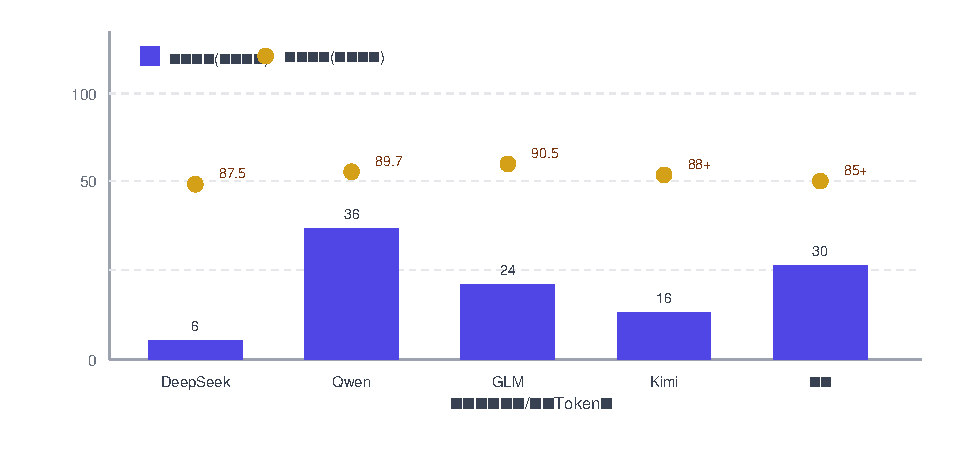
\includegraphics[width=0.92\linewidth]{figures/fig-di-si-shi-er-zhang-1}
\\[2pt]\small 圖 4：五款模型的價格與效能對比（價格越低越好，得分越高越好）
\end{center}

\booksection{三、模型選擇決策框架}

瞭解了各模型的特點後，如何為自己的專案選模型？這裡送你一套“四問決策法”——回答四個問題，就能鎖定最適合你的模型。

你的專案在國內還是國際部署？

國內 選國產模型

|

國際 可選海外模型

核心任務是程式設計還是其他？

程式設計 Claude 或 DeepSeek

|

其他 繼續判斷

需要超長上下文(>50萬Token)？

需要 Gemini 或 Kimi

|

不需要 繼續判斷

預算敏感嗎？

敏感 DeepSeek 或 Qwen-turbo

|

不敏感 GPT-5.6 或 Claude

\begin{center}\small\color{gray}圖 5：大型語言模型選擇四問決策法\end{center}

\begin{tcbinfo}{小貼士：組合策略}
這個決策法不是教條——很多場景需要組合使用多個模型。一個常見的組合策略：用 DeepSeek 或 Qwen 做日常開發（成本低、中文好），用 Claude 做關鍵架構設計（推理強、幻覺低），用 Gemini 做多模態分析（影像影片處理）。按需切換模型，而不是“一個模型用到死”。

\end{tcbinfo}

\booksection{四、API 呼叫入門：從零開始接入大型語言模型}

很多 AI 程式設計教學只教你怎麼用對話介面，但真正的“AI 程式設計”——讓你的應用呼叫大型語言模型——需要透過 API。API（Application Programming Interface，應用程式設計介面）是程式之間的通訊協議。透過 API，你的程式碼可以像呼叫一個函式一樣，呼叫大型語言模型的能力。

\booksubsection{什麼是 Token}

在瞭解 API 之前，必須先理解 “Token” 這個概念。Token 是大型語言模型計費的基本單位，可以理解為 “AI 的閱讀和寫作單位”。一個 Token 大約對應：英文中 0.75 個單詞（4 個字元），中文中 0.5-1 個漢字。一段 1000 字的中文文字，大約消耗 1500-2000 個 Token。

Token 不是字數，也不是字元數。大型語言模型使用專門的分詞器（Tokenizer）將文字切分成 Token。同一個詞在不同模型中的 Token 數量可能不同——比如“人工智慧”在 GPT 中可能是 3 個 Token，在 DeepSeek 中可能是 2 個。大多數模型的 API 會返回實際消耗的 Token 數量，你可以在 API 響應中檢視。

\begin{tcbinfo}{Token 成本快速估算}
100 萬字中文約等於 150 萬 Token。用 DeepSeek V4 Flash 處理 100 萬字輸入 + 100 萬字輸出，成本約 0.42 美元（約 3 元人民幣）；用 Claude Fable 5 處理同樣的量，成本約 60 美元（約 434 元人民幣）。這就是為什麼模型選擇直接影響你的專案成本。

\end{tcbinfo}

\booksubsection{獲取 API Key}

使用大型語言模型 API 的第一步是獲取 API Key——一串用於身份驗證的金鑰。每個模型提供商都有自己的 API 平臺，你需要註冊帳號並建立 API Key。以下是主流模型的 API 平臺入口和獲取流程：

\begin{center}
\begin{tabularx}{\linewidth}{|X|X|X|X|}
\hline
\textbf{模型} & \textbf{API 平臺} & \textbf{獲取流程} & \textbf{免費額度} \tabularnewline
\hline
DeepSeek & platform.deepseek.com & 註冊 實名認證 建立 API Key & 新使用者贈送額度 \tabularnewline
通義千問 & bailian.aliyun.com（百鍊平臺） & 阿里雲帳號登入 開通服務 建立 Key & 新使用者免費試用 \tabularnewline
智譜GLM & open.bigmodel.cn & 註冊 實名認證 建立 API Key & 新使用者贈送額度 \tabularnewline
Kimi & platform.moonshot.cn & 註冊 實名認證 建立 API Key & 有限免費額度 \tabularnewline
豆包 & volcengine.com（火山引擎） & 註冊 開通方舟 建立 API Key & 註冊送大量 Token \tabularnewline
OpenAI GPT & platform.openai.com & 註冊 繫結信用卡 建立 API Key & 無免費額度(需付費) \tabularnewline
Anthropic Claude & console.anthropic.com & 註冊 綁卡 建立 API Key & 新使用者少量額度 \tabularnewline
\hline
\end{tabularx}
\end{center}

\begin{center}\small\color{gray}主流模型 API 平臺及 Key 獲取方式（2026 年 8 月）\end{center}

\textbf{安全提示：API Key = 錢包密碼}\par

API Key 等同於你的錢包密碼——任何拿到 Key 的人都可以用你的額度呼叫模型。因此：永遠不要把 API Key 寫在程式碼中（用環境變數管理）；永遠不要把含 Key 的程式碼提交到公開的 Git 倉庫；永遠不要在社交媒體分享含 Key 的截圖。如果 Key 洩露了，立即在平臺上刪除並重新增立。

\booksubsection{第一次 API 呼叫}

獲取 API Key 後，你可以用任何程式語言呼叫大型語言模型 API。以下用 Python 示範一個最簡單的呼叫——向 DeepSeek 傳送一條訊息並獲取回覆。

\begin{lstlisting}[language=Python]
# 安裝SDK：pip install openai
# DeepSeek相容OpenAI SDK格式，可以直接用
from openai import OpenAI
import os

# 1. 建立客戶端（API Key從環境變數讀取）
client = OpenAI(
    api_key=os.environ.get("DEEPSEEK_API_KEY"),
    base_url="https://api.deepseek.com"
)

# 2. 傳送請求
response = client.chat.completions.create(
    model="deepseek-chat",  # 指定模型
    messages=[
        {"role": "system", "content": "你是一個Python程式設計助手。"},
        {"role": "user", "content": "寫一個快速排序函式。"}
    ]
)

# 3. 獲取回覆
print(response.choices[0].message.content)

# 4. 檢視Token消耗
print(f"輸入Token: {response.usage.prompt_tokens}")
print(f"輸出Token: {response.usage.completion_tokens}")
print(f"總Token: {response.usage.total_tokens}")
\end{lstlisting}

這段程式碼的核心邏輯是：建立使用者端（攜帶 API Key 和模型地址） 構造訊息列表（system 設定角色，user 是使用者輸入） 傳送請求 獲取回覆。這個模式幾乎適用於所有相容 OpenAI 格式的模型——只需要更換 api\_key 和 base\_url 就能切換模型。這就是為什麼很多國產模型選擇相容 OpenAI SDK 格式：開發者只需改兩行程式碼就能切換模型，遷移成本極低。

以下是切換到其他模型的程式碼差異——注意只需要改兩行：

\begin{lstlisting}[language=Python]
# DeepSeek
client = OpenAI(
    api_key=os.environ.get("DEEPSEEK_API_KEY"),
    base_url="https://api.deepseek.com"
)
# model="deepseek-chat"

# 通義千問（百鍊平臺）
client = OpenAI(
    api_key=os.environ.get("DASHSCOPE_API_KEY"),
    base_url="https://dashscope.aliyuncs.com/compatible-mode/v1"
)
# model="qwen-plus"

# 智譜GLM
client = OpenAI(
    api_key=os.environ.get("GLM_API_KEY"),
    base_url="https://open.bigmodel.cn/api/paas/v4"
)
# model="glm-4"

# OpenAI GPT
client = OpenAI(
    api_key=os.environ.get("OPENAI_API_KEY"),
    # base_url使用預設值即可
)
# model="gpt-5.6-terra"
\end{lstlisting}

\booksubsection{流式響應處理}

在實際應用中，你通常不希望等 AI 寫完所有內容才一次性顯示——那會讓使用者等太久。流式響應（Streaming）可以讓你在 AI 生成的同時逐字顯示，大幅提升使用者體驗。就像打字機一樣，字一個一個蹦出來，使用者的感覺是完全不同的。

\begin{lstlisting}[language=Python]
# 流式響應：逐字輸出
stream = client.chat.completions.create(
    model="deepseek-chat",
    messages=[
        {"role": "user", "content": "寫一個Python的氣泡排序教程"}
    ],
    stream=True  # 開啟流式響應
)

# 逐塊接收並列印
for chunk in stream:
    if chunk.choices[0].delta.content is not None:
        print(chunk.choices[0].delta.content, end="", flush=True)
# 輸出會像打字機一樣逐字顯示
\end{lstlisting}

\booksection{五、Token Plan 購買指南}

大多數模型提供商有兩種計費方式：按量計費（Pay-as-you-go）和資費方案訂閱（Token Plan / Subscription）。理解這兩種方式的區別，能幫你大幅降低使用成本。

\booksubsection{按量計費 vs 資費方案訂閱}

\begin{center}
\begin{tabularx}{\linewidth}{|X|X|X|}
\hline
\textbf{維度} & \textbf{按量計費(Pay-as-you-go)} & \textbf{資費方案訂閱(Subscription)} \tabularnewline
\hline
計費方式 & 用多少Token付多少錢 & 預付固定費用，獲得額度 \tabularnewline
適合場景 & 使用量不穩定、偶爾呼叫 & 使用量穩定、高頻呼叫 \tabularnewline
價格優勢 & 標準價 & 比按量低20\%-50\% \tabularnewline
靈活性 & 隨時可用，無需承諾 & 需要預付，額度過期可能作廢 \tabularnewline
超額處理 & 自動按量計費 & 超出額度後轉為按量計費 \tabularnewline
代表平臺 & 各模型官方API平臺 & OpenAI Plus/Pro, Claude Pro, Cursor Pro \tabularnewline
\hline
\end{tabularx}
\end{center}

\begin{center}\small\color{gray}兩種計費方式的對比\end{center}

對於初學者，建議從按量計費開始——不需要預付費用，用多少花多少。當你的月使用量穩定在一個水準後（比如每月超過 50 元），再考慮切換到資費方案訂閱以獲得更低單價。

\booksubsection{主流訂閱資費方案一覽}

\begin{center}
\begin{tabularx}{\linewidth}{|X|X|X|X|}
\hline
\textbf{資費方案} & \textbf{月費} & \textbf{包含內容} & \textbf{適合人群} \tabularnewline
\hline
ChatGPT Free & 免費 & GPT-5.6 Luna 無限文字對話 & 零基礎體驗 \tabularnewline
ChatGPT Plus & US\$20/月 & GPT-5.6 Sol、影像生成、資料分析、外掛訪問 & 中度使用者 \tabularnewline
ChatGPT Pro & US\$200/月 & 無限制使用所有模型、優先訪問新功能 & 重度專業使用者 \tabularnewline
Claude Free & 免費 & 有限次數Claude對話 & 零基礎體驗 \tabularnewline
Claude Pro & US\$20/月 & 無限制Claude使用、優先訪問新模型 & 程式設計開發者 \tabularnewline
Cursor Free & 免費 & 有限次數AI補全和對話 & 初學者體驗 \tabularnewline
Cursor Pro & US\$20/月 & 無限AI補全、500次/月進階請求 & 日常開發者 \tabularnewline
Cursor Business & US\$40/月/人 & 團隊協作、管理後臺、隱私模式 & 團隊使用 \tabularnewline
\hline
\end{tabularx}
\end{center}

\begin{center}\small\color{gray}主流 AI 工具訂閱資費方案（2026 年 8 月）\end{center}

國內模型的訂閱方案略有不同。DeepSeek 主要按量計費，沒有月度訂閱資費方案——你充值後按實際使用量扣費。通義千問在百鍊平臺提供預付費資源包（購買一定量的 Token 額度，享受折扣價）。豆包在火山引擎上也有類似的預付費方案。對於國內開發者，最經濟的組合通常是：DeepSeek 按量計費（日常開發）+ 豆包免費額度（體驗測試）。

\booksubsection{API 聚合平臺}

如果你需要同時使用多個模型，API 聚合平臺是一個省心的選擇。聚合平臺提供一個統一的 API Key，你就能呼叫全球幾十種模型，無需在每個平臺分別註冊。

\begin{center}
\begin{tabularx}{\linewidth}{|X|X|X|X|}
\hline
\textbf{平臺} & \textbf{特點} & \textbf{價格優勢} & \textbf{適合場景} \tabularnewline
\hline
OpenRouter (openrouter.ai) & 海外聚合平臺，一個Key呼叫全球模型 & 價格透明，支援實時比價 & 需要靈活切換多個海外模型 \tabularnewline
SiliconFlow (siliconflow.cn) & 國內聚合平臺，提供多種國產模型API & 比官方低20\%-30\% & 國內開發者，多模型比價 \tabularnewline
Azure OpenAI (微軟代理) & 微軟Azure代理的OpenAI API & Batch API可打5折 & 企業級OpenAI呼叫，大批次非同步任務 \tabularnewline
百度千帆 (qianfan.baidubce.com) & 百度AI雲平臺，提供文心等模型 & 新使用者贈送額度 & 百度生態使用者 \tabularnewline
\hline
\end{tabularx}
\end{center}

\begin{center}\small\color{gray}主流 API 聚合平臺（2026 年 8 月）\end{center}

\textbf{避坑提醒：別買“共享 Key”}\par

不要在淘寶、閒魚等平臺購買所謂的“共享 API Key”——這些 Key 通常來路不明，可能隨時被封號，還有資料洩露風險。始終透過官方平臺或正規聚合平臺獲取 API Key。

\booksubsection{成本最佳化策略}

選對模型只是第一步，如何“用得省錢”同樣重要。以下是幾個經過實踐驗證的成本最佳化策略：

\begin{enumerate}
  \item 善用快取命中。很多模型提供"快取"功能——當你的請求中包含之前已經處理過的內容（如系統提示詞），這部分只按極低價格計費。DeepSeek 的快取命中價格僅為普通價格的 1/60。把固定的系統提示放在訊息列表開頭，可以最大化快取命中。
  \item 分級路由——用便宜模型處理簡單任務，貴模型處理複雜任務。比如用 DeepSeek V4 Flash 做文字分類（輸出 2 元/百萬 Token），用 Claude 做架構設計（輸出 181 元/百萬 Token）。一個專案裡 80\% 的呼叫可以用便宜模型。
  \item 限制輸出長度。API 按輸出 Token 計費，輸出越長越貴。在不需要長篇大論的場景中，設定 max\_tokens 引數限制輸出長度，避免 AI"廢話太多"。
  \item 使用 Batch API 處理非實時任務。如果你有大量不需要即時響應的任務（如批次資料標註、檔案摘要），使用 Batch API 可以享受 50\% 折扣。OpenAI 和 Azure 都提供這個功能。
  \item 監控 Token 用量。大多數 API 平臺提供用量統計面板。定期檢視用量分佈，找出消耗 Token 最多的呼叫，針對性最佳化。一個小小的 Prompt 調整（比如把"請詳細解釋"改成"請用 3 句話解釋"）可能節省 50\% 的 Token。
\end{enumerate}

\begin{center}
\begin{tabularx}{\linewidth}{|X|X|X|X|}
\hline
\textbf{最佳化策略} & \textbf{節省幅度} & \textbf{實施難度} & \textbf{說明} \tabularnewline
\hline
快取命中 & 最高98\% & 低 & 把固定內容放在訊息開頭 \tabularnewline
分級路由 & 50\%-80\% & 中 & 簡單任務用便宜模型 \tabularnewline
限制輸出長度 & 30\%-60\% & 低 & 設定max\_tokens引數 \tabularnewline
Batch API & 50\% & 低 & 非實時任務用批處理 \tabularnewline
Prompt最佳化 & 20\%-50\% & 中 & 精簡Prompt，減少冗餘 \tabularnewline
\hline
\end{tabularx}
\end{center}

\begin{center}\small\color{gray}成本最佳化策略及效果（2026 年 8 月）\end{center}

\booksection{六、實戰：在專案中接入大型語言模型 API}

讓我們用一個完整的實戰來結束本章——建立一個 “AI 摘要生成器”：使用者輸入一段長文字，呼叫大型語言模型 API 生成摘要。這個實戰會展示 API 呼叫的完整流程：環境配置、API 呼叫、錯誤處理、成本控制。

\begin{lstlisting}[language=Python]
# ai_summarizer.py - AI摘要生成器
import os
from openai import OpenAI

# 1. 配置（API Key從環境變數讀取，絕不硬編碼）
client = OpenAI(
    api_key=os.environ.get("DEEPSEEK_API_KEY"),
    base_url="https://api.deepseek.com"
)

def summarize(text: str, max_length: int = 200) -> dict:
    """生成文字摘要

    Args:
        text: 要摘要的原文
        max_length: 摘要最大長度（Token數）

    Returns:
        dict: 包含摘要和Token消耗資訊
    """
    try:
        response = client.chat.completions.create(
            model="deepseek-chat",
            messages=[
                {
                    "role": "system",
                    "content": "你是一個摘要生成器。"
                               "請用簡潔的中文總結使用者提供的文字。"
                               "摘要不超過3句話。"
                },
                {
                    "role": "user",
                    "content": f"請摘要以下文字:\n\n{text}"
                }
            ],
            max_tokens=max_length,  # 限制輸出長度
            temperature=0.3  # 低溫度=更穩定
        )

        return {
            "success": True,
            "summary": response.choices[0].message.content,
            "input_tokens": response.usage.prompt_tokens,
            "output_tokens": response.usage.completion_tokens,
            "total_tokens": response.usage.total_tokens
        }

    except Exception as e:
        return {
            "success": False,
            "error": str(e)
        }

# 2. 使用示例
if __name__ == "__main__":
    long_text = """
    （貼上一段長文字...）
    """

    result = summarize(long_text)

    if result["success"]:
        print(f"摘要: {result['summary']}")
        print(f"消耗Token: {result['total_tokens']}")
        # 估算成本：DeepSeek V4 Flash
        cost = result['total_tokens'] * 0.000004  # 約0.4分/千Token
        print(f"預估成本: {cost:.4f}元")
    else:
        print(f"出錯了: {result['error']}")
\end{lstlisting}

這段程式碼體現了 API 呼叫的幾個最佳實踐：API Key 透過環境變數讀取，絕不硬編碼在程式碼中；函式有清晰的檔案和型別提示；設定了 max\_tokens 限制輸出長度；temperature 設為低值（0.3）以獲得更穩定的輸出；有完整的錯誤處理；返回 Token 消耗資訊用於成本追蹤。當你用 AI 來寫這段程式碼時，可以告訴它這些要求——它完全有能力幫你實現。

本章的最終啟示：模型是"彈藥"，方法論是"戰術"。選對彈藥能讓戰鬥更順利，但沒有好的戰術，再好的彈藥也打不贏仗。瞭解了各模型的特點和 API 使用方法後，你就有了一個充足的"彈藥庫"——但怎麼打這場仗，還是要靠前幾章學到的思維方法論。

\begin{tcbpractice}{來動手：跑通你的第一次 API 呼叫}
註冊一個國產模型平臺（推薦 DeepSeek 或智譜，都送新使用者額度），建立 API Key，把它寫進系統環境變數（而不是程式碼裡！），然後執行上面“第一次 API 呼叫”的程式碼。看到 AI 的回覆列印出來的那一刻，你就跨過了“用 AI”和“造 AI 應用”之間的分界線。

\end{tcbpractice}

\begin{tcbsummary}{本章小結}
\begin{itemize}
  \item 國際三強：GPT-5.6（均衡全能）、Claude（程式設計天花板+幻覺率僅1\%）、Gemini（多模態之王+200萬上下文）
  \item 國產五強：DeepSeek V4（價效比之王，注意漲價公告）、Qwen3.7（企業級）、GLM-5.1（SWE國產第一）、Kimi K3（超長文字）、豆包（免費入門）
  \item 四問決策法：部署地點？程式設計還是其他？超長上下文？預算敏感？
  \item Token 是計費單位：中文 1 字約 1.5-2 Token；100萬字約150萬Token
  \item API Key = 錢包密碼：環境變數管理，絕不硬編碼、不上傳Git
  \item 國產模型普遍相容 OpenAI SDK：換模型只需改 api\_key 和 base\_url 兩行
  \item 省錢五招：快取命中、分級路由、限制輸出、Batch API、監控用量
\end{itemize}

\end{tcbsummary}
